% Autor: Elias Welt
\section{Das Dashboard -- Zentrale Übersichtsansicht}

Die Startseite der Anwendung, realisiert in der Komponente \texttt{MainDashboard.jsx}, stellt nach erfolgreicher Authentifizierung den primären Einstiegspunkt für den Nutzer dar. Sie verfolgt das Konzept eines persönlichen Lernportals, das auf einen Blick die relevantesten Informationen und die häufigsten Aktionen bündelt.

\begin{figure}[h]
    \centering
    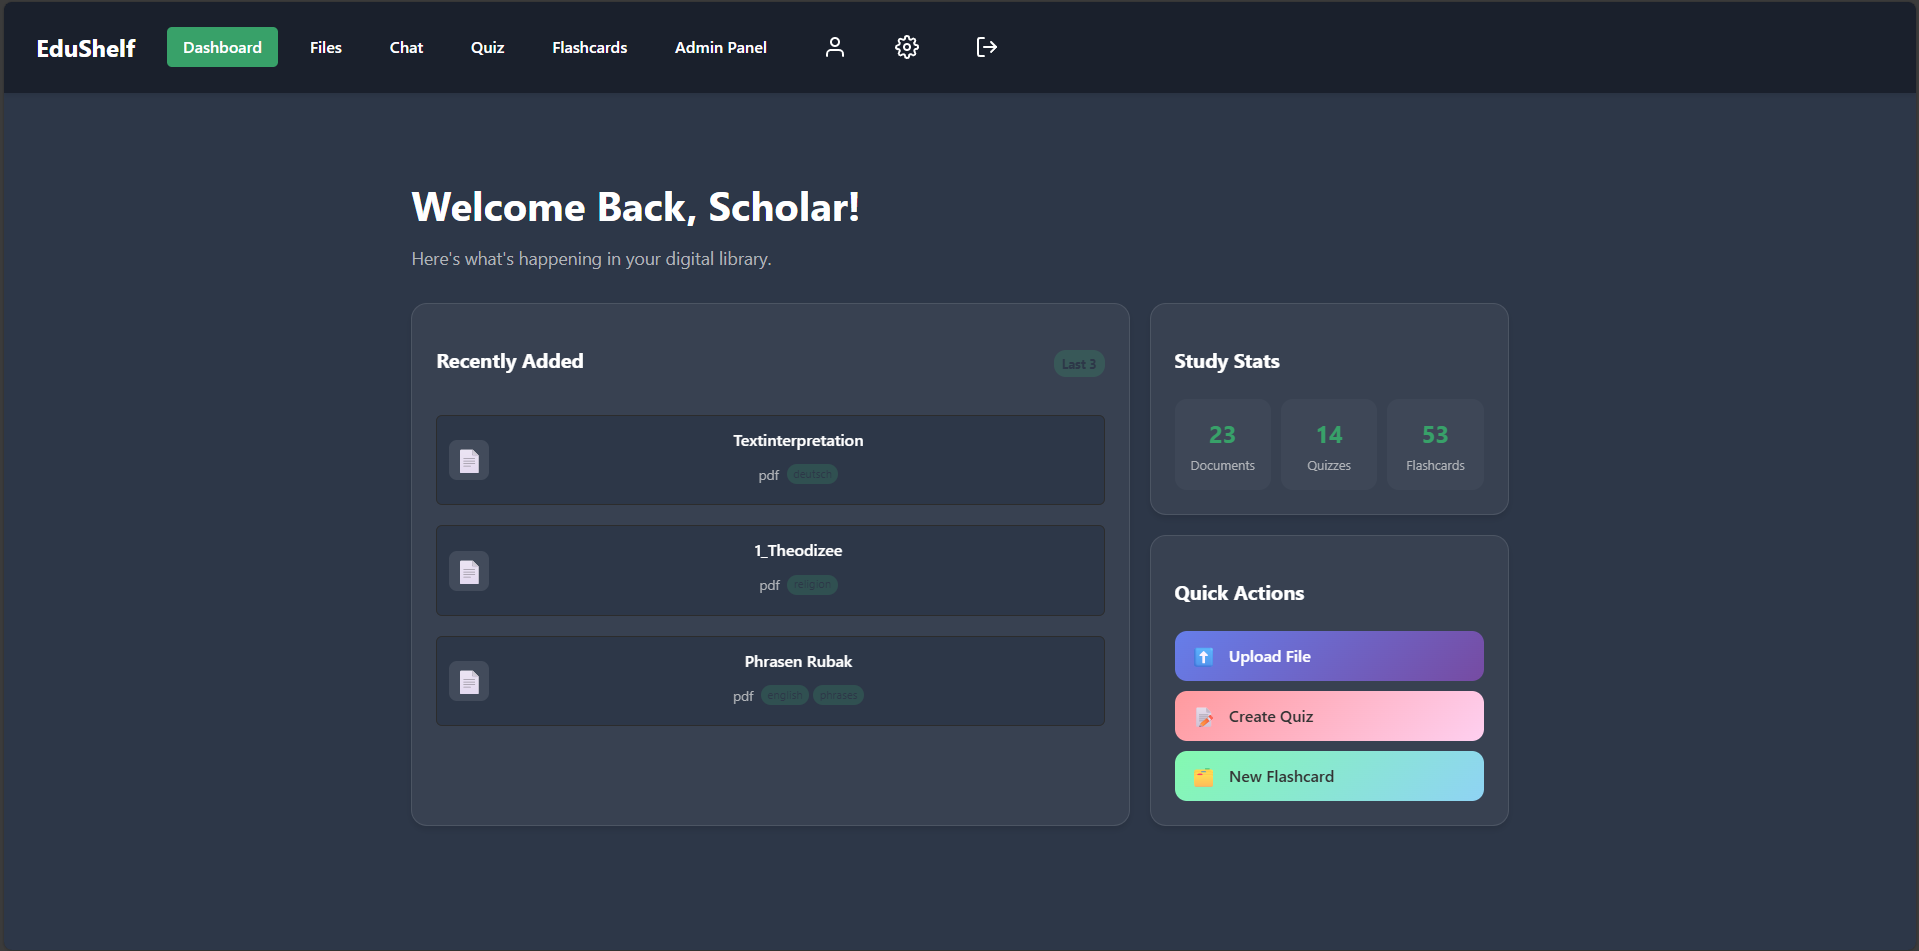
\includegraphics[width=0.92\textwidth]{img/dashboard-dark-mode}
    \caption{Hauptdashboard von EduShelf im Dark-Mode}
    \label{fig:dashboard}
\end{figure}

\subsection{Architektur und Datenladen}

Ein zentrales Designprinzip des Dashboards ist das parallele Laden aller benötigten Daten. Anstatt Dokumente, Quiz-Einträge und Lernkarten sequenziell abzurufen -- was die Ladezeit mit jeder weiteren Anfrage erhöhen würde -- wird \texttt{Promise.all()} eingesetzt. Diese Methode startet alle asynchronen Anfragen gleichzeitig und wartet, bis die langsamste von ihnen abgeschlossen ist.

\begin{lstlisting}[language=JavaScript, caption={Paralleles Datenladen mit Promise.all im Dashboard}]
const fetchData = async () => {
  try {
    const [docsData, quizzes, flashcards] = await Promise.all([
      getDocuments(),
      getQuizzes(),
      getFlashcards()
    ]);
    // Alle Daten sind gleichzeitig verfuegbar
    setStats({
      documents: docsData.totalCount || docs.length,
      quizzes:   quizzes.totalCount   || quizzes.length,
      flashcards: flashcards.totalCount || flashcards.length
    });
  } catch (error) {
    console.error('Error fetching dashboard data:', error);
  }
};
\end{lstlisting}

Das Ergebnis ist eine messbar kürzere Wartezeit im Vergleich zu sequenziellen Aufrufen, da die Gesamtdauer der Nettozeit der langsamsten Einzelanfrage entspricht, nicht der Summe aller Anfragen.

\subsection{Filterung geteilter Dateien}

Das Dashboard implementiert eine clientseitige Filterlogik für geteilte Dateien. Da Dokumente, die von anderen Nutzern geteilt wurden, zunächst im Zustand \textit{ausstehend} verbleiben, werden nur jene Dokumente in der Übersicht angezeigt, die der Nutzer explizit akzeptiert hat. Die Entscheidungen des Nutzers (akzeptiert oder abgelehnt) werden im \texttt{localStorage} persistiert und beim Laden ausgewertet:

\begin{lstlisting}[language=JavaScript, caption={Filterung von Shared Files anhand des localStorage-Status}]
const acceptedShares = JSON.parse(
  localStorage.getItem('edushelf_accepted_shares') || '[]'
);
const rejectedShares = JSON.parse(
  localStorage.getItem('edushelf_rejected_shares') || '[]'
);

docs = docs.filter(doc => {
  if (!doc.isShared) return true;        // eigene Dateien immer anzeigen
  if (rejectedShares.includes(doc.id)) return false; // abgelehnte ausblenden
  return acceptedShares.includes(doc.id);  // nur akzeptierte zeigen
});
\end{lstlisting}

\subsection{Schnellaktionen und Statistik-Widget}

Das Dashboard gliedert sich in drei funktionale Bereiche:

\begin{enumerate}
    \item \textbf{Recently Added}: Zeigt die drei zuletzt hochgeladenen Dokumente mit Dateiname, Typ und zugewiesenen Tags an. Ein Klick öffnet die Inline-Vorschau über \texttt{FileViewer}.
    \item \textbf{Study Stats}: Zeigt aggregierte Zählwerte für Dokumente, Quizzes und Lernkarten. Diese Statistiken werden bei jeder Aktion (Upload, Erstellen, Löschen) durch erneuten Aufruf von \texttt{fetchData()} aktualisiert.
    \item \textbf{Quick Actions}: Drei Schaltflächen ermöglichen das unmittelbare Erstellen eines Uploads, eines Quiz oder einer Lernkarte, ohne dass dafür die entsprechende Unterseite aufgerufen werden muss. Die zugehörigen Modaldialoge werden direkt im Dashboard-Kontext gerendert.
\end{enumerate}

Dieses Konzept minimiert die Anzahl der notwendigen Navigationsschritte für häufig ausgeführte Aktionen und entspricht der Zielsetzung einer effizienten Lernoberfläche.
